\documentclass{article}[18pt]
\usepackage{../../../../format}
\lhead{Networks and Systems - Security}


\begin{document}
\begin{center}
\underline{\huge Identification, authentication, authorization}
\end{center}
\section{Access Control}
Access to the resources:
\begin{itemize}
	\item Claim the identity
	\item Verify the credentials
	\item Check permissions
	\item Grant access
\end{itemize}
\section{Identification}
\begin{defin}[Subject]
An active entity within a system (physical person, script, etc)	
\end{defin}
\begin{defin}[Principal]
An entity that can be granted access (represented by a username, userid, pin etc)
\end{defin}
The subject identifies itself to the system as a principal
\section{Authentication}
The system verifies the identity of the user
\begin{defin}[Object]
Resource that some principals may access or use
\end{defin}
The system checks that the principal has the permissions to access an object
\section{Credentials}
\begin{itemize}
	\item What do you know? Passwords, PINs
	\item What do you have? Authentication key, passport, ticket, mobile phone
	\item Who you are? Biometrics
\end{itemize}
\section{Passwords}
Common Security Guidelines:
\begin{itemize}
	\item Adopt long passphrases
	\item Avoid easy to guess passwords
	\item Use combination of a-z, A-Z, 0-9 and symbols
	\item Do not write down passwords
	\item Avoid using the same password for multiple services
\end{itemize}
However - when internet users log on to as many as 25 password-protected sites per day, remembering a different and secure password for each one is very difficult.\\
Passwords should be stored in a password manager so you only have to remember one secure password
\section{Authentication Keys}
Authentication keys (e.g. SSH keys)
\begin{itemize}
	\item Similar to passwords, but
	\item RSA-based keys
	\item Subject create private/public key
	\item Share the public key with services
	\item Per device RSA key
\end{itemize}
Advantages:
\begin{itemize}
	\item Public key leak are inconsequential
	\item Compromised device access can be revoked
\end{itemize}
\section{Security Keys}
Authentication keys weakness: Compromised client\\
\\
Solution: Physical security keys:
\begin{itemize}
	\item Static password token (not recommended)
	\item Asynchronous tokens (one-time passwords)
	\item Challenge-response tokens
\end{itemize}
\section{Biometrics}
\textbf{Advantages}:
\begin{itemize}
	\item Non-repudiation: a way to guarantee that an individual who accesses a certain facility cannot later deny using it
\end{itemize}
\textbf{Disadvantages}:
\begin{itemize}
	\item Uncertainty: Compromise between false-positive and false-negatives
\end{itemize}
Receiver Operating Characteristic (ROC) curve
\begin{center}
	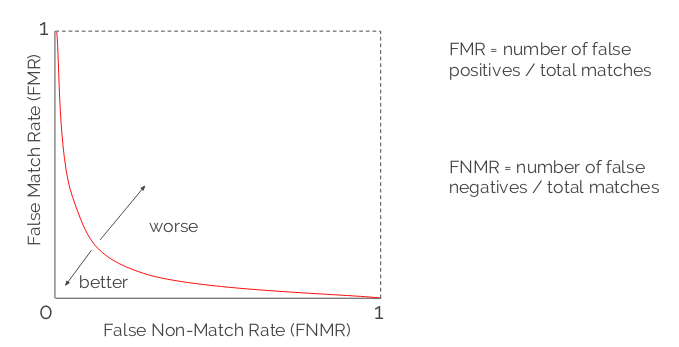
\includegraphics[scale=0.7]{ROC}
\end{center}
Performance policy
\begin{itemize}
	\item Prefer low FMR. E.g. automatic border control. Refer to human on negative result
	\item Prefer low FNMR. E.g. suspect recognition on CCTV. Refer to human on positive result
\end{itemize}
\section{Two-factor authentication}
Two-factor authentication.\\
\\
Combine two authentication factors from:
\begin{itemize}
	\item What you know: password, pin
	\item What you have: mobile phone, authentication key
\end{itemize}
\section{Zero-Knowledge Password Proof}
\textbf{Objective}: Do not reveal anything in the client/server communications about the password.\\
Otherwise we are vulnerable to replay attacks.\\
\\
Most common ZKPP approach: Challenge-response auth:
\begin{itemize}
	\item Serer generate unique challenge value: nonce
	\item Server send nonce to the client
	\item Client computer response = hash(nonce + password)
	\item Client send response back to server
	\item Server compare the response with hash(nonce+stored password)
\end{itemize}
Nonce properties:
\begin{itemize}
	\item Nonce: Random or pseudo-random unique value
	\item Uniqueness: Prevent replay attacks
	\item Susceptible to PRNG flaws
\end{itemize}
\section{Example: EMV Payment}
\begin{itemize}
	\item Standard used for all credit cards
	\item EMV standard: Initially written in 1993
	\item Over 3600 pages of protocol specification
	\item Requirements varies from bank to bank
\end{itemize}
Card authentication mechanism
\begin{itemize}
	\item Static data authentication (offline)
	\item Dynamic data authentication (offline)
	\item Combined DDA with application cryptogram generation (offline)
	\item Cryptogram (online)
\end{itemize}
Multiple cardholder verification mechanism (CVM)
\begin{itemize}
	\item No CVM required (e.g motorway toll)
	\item Signature (common in some countries, e.g. US)
	\item Offline pin (no internet, pin verified by the card)
	\item Online PIN (internet, pin verified by the bank)
\end{itemize}
\subsection{SDA: Static Data Authentication}
\begin{itemize}
	\item Offline card payment
	\item Used by old card and terminal
	\item Lowest common denominator
	\item Vulnerable to skimming attack
	\item During transaction, terminal records the static data
	\item A cloned card is created with the same static data
\end{itemize}
\begin{center}
	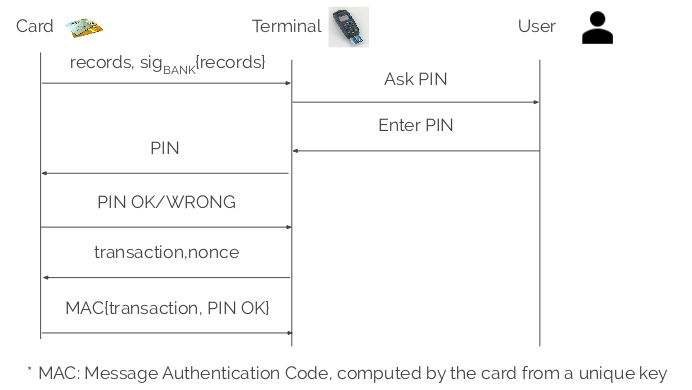
\includegraphics[scale=0.7]{EMV}
\end{center}
An attacker can get records, $sig_{BANK}[records]$ by listening to a valid transaction\\
\\
The the attacker can create a fake card using $sig_{BANK}[records]$ and generate an invalid MAC. For offline transaction, the merchant cannot verify the MAC anyway. By the time the merchant sends the transactions to the bank, the attacker will be long gone\\
\\
Problem: static password
\subsection{DDA: Dynamic Data Authentication}
Use challenge-response authentication to generate data unique to the transaction
\begin{center}
	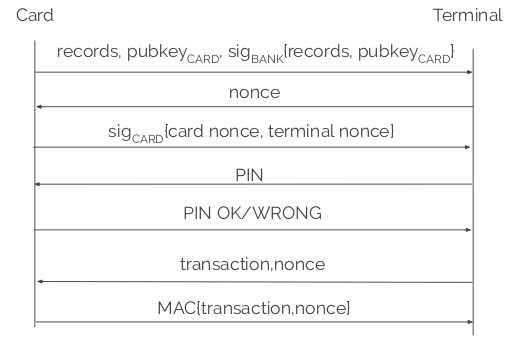
\includegraphics[scale=0.7]{dd}
\end{center}
Card clone is not possible because sig$_{card}$[card nonce, terminal nonce] is different at every transaction.\\
\\
However, card answer to PIN check is not authenticated either\\
\\
A wedge between a stolen card and a terminal can pretend that the password is always correct
\begin{center}
	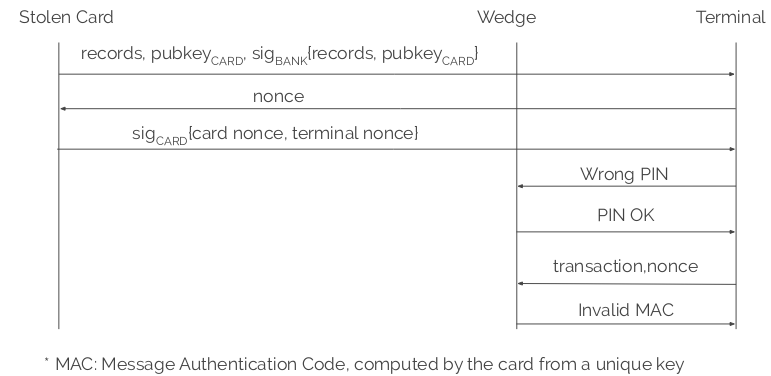
\includegraphics[scale=0.7]{DDA2}
\end{center}
\subsection{CDA: Combined DDA/Application Cryptogram Generation}
Solution: Second card authentication step after PIN check\\
\\
The terminal sends a message called CVMR representing the terminal view of the operation (PIN OK, PIN Wrong, signature etc) for the card to compare with its own point of view
\begin{center}
	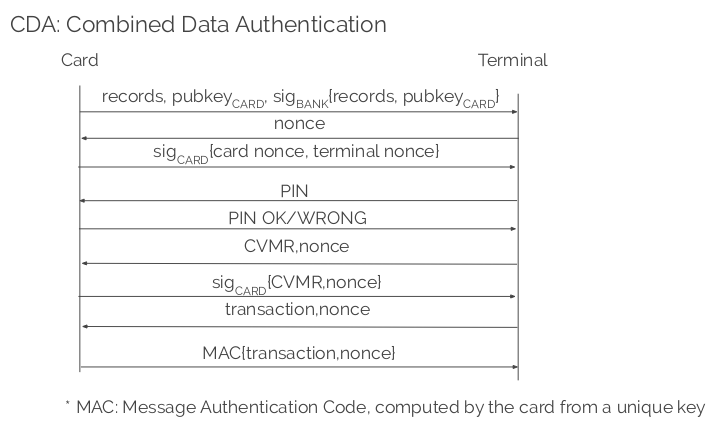
\includegraphics[scale=0.7]{CDA}
\end{center}
Takeaway:
\begin{itemize}
	\item Do not send static auth data (e.g. unencrypted passwords)
	\item Use challenge-response to prevent replay attacks
	\item Make sure that authentication is verified at all steps
\end{itemize}
\end{document}